% 90-14(90쪽) — 전체집합 U 안의 두 진리집합 P, Q 벤 다이어그램. 타원 Q 안에 타원 P 가 들어 있고 P 안에 a·b, Q 안 P 밖에 c·d, U 안 Q 밖에 e 가 있다.
% 스캔 화질이 낮아 TikZ 로 다시 그림. 라벨은 원문 그대로 U·Q·P 와 원소 다섯 개만 둔다 — 보기 ①~⑤ 중 어느 것이 답인지는 그림에 적지 않는다.
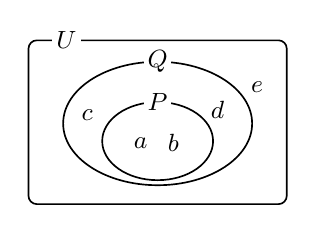
\begin{tikzpicture}[scale=0.8, line width=0.5pt, every node/.style={font=\small}]
  \draw[line width=0.6pt, rounded corners=3pt] (-2.05,-1.3) rectangle (2.05,1.3);
  \node[fill=white, inner sep=1.5pt] at (-1.45,1.3) {$U$};
  \draw[line width=0.6pt] (0,-0.02) ellipse (1.5 and 0.98);
  \draw[line width=0.6pt] (0,-0.30) ellipse (0.88 and 0.62);
  \node[fill=white, inner sep=1.2pt] at (0,0.96) {$Q$};
  \node[fill=white, inner sep=1.2pt] at (0,0.32) {$P$};
  \node at (-1.12,0.12) {$c$};
  \node at (-0.27,-0.33) {$a$};
  \node at (0.25,-0.33) {$b$};
  \node at (0.95,0.20) {$d$};
  \node at (1.58,0.56) {$e$};
\end{tikzpicture}
